\documentclass{article}
\usepackage{graphicx}
\usepackage{amsmath}
\usepackage{hyperref}
\usepackage{geometry}
\geometry{a4paper, margin=1in}

\title{Ergodic Engine Upgrade: \\ Deterministic Weaving of the $4f$ Orbital}
\author{Daniel Gezin \\ \href{https://orcid.org/0009-0003-7309-7050}{ORCID: 0009-0003-7309-7050}}
\date{\today}

\begin{document}
\maketitle

\section{Introduction}
The Topological Geon framework redefines particles not as zero-dimensional points, but as macroscopic topological structures (Möbius loops and knots) confined by the Casimir vacuum pressure. In our latest WebGL simulation upgrade, we successfully moved beyond deterministic sine-wave "wobbles" and hardcoded orbital steering to a fully integrated \textbf{Hamiltonian emergence}.

\section{The Nodal Trap and The Ergodic Breakthrough}
When simulating complex orbitals like the $4f$ ($n=4, l=3, m=2$), the electron must traverse a volume separated by quantum nodes (regions of zero probability).

\subsection{Quantum Potential ($V_Q$)}
In our physics integration, the electron is deterministically steered by the spatial gradient of the Quantum Potential:
\begin{equation}
    V_Q = -\frac{\hbar^2}{2m} \frac{\nabla^2 R}{R}
\end{equation}
While this correctly shapes the probability density, it creates infinite repulsive walls at the nodal boundaries, permanently trapping the electron in a single orbital lobe.

\subsection{The Langevin Thermostat (ZPF Heat)}
To allow the deterministic path to fully weave the required 3D geometric volume (the Schrödinger cloud), we introduce the physical \textbf{Zero-Point Fluctuations (ZPF)} of the hyper-elastic vacuum fluid via a Langevin Thermostat.

By injecting a calibrated stochastic kinetic kick (e.g., $ZPF = 4.7$), the electron gains the precise momentum required to breach the nodal barrier and achieve macroscopic ergodicity, resolving the Nodal Trap problem.

\section{Simulation Results}
Below is a high-resolution frame of the WebGL simulation demonstrating the successful deterministic traversal of the $4f$ orbital state over 6.71 million timesteps.

\begin{figure}[h!]
    \centering
    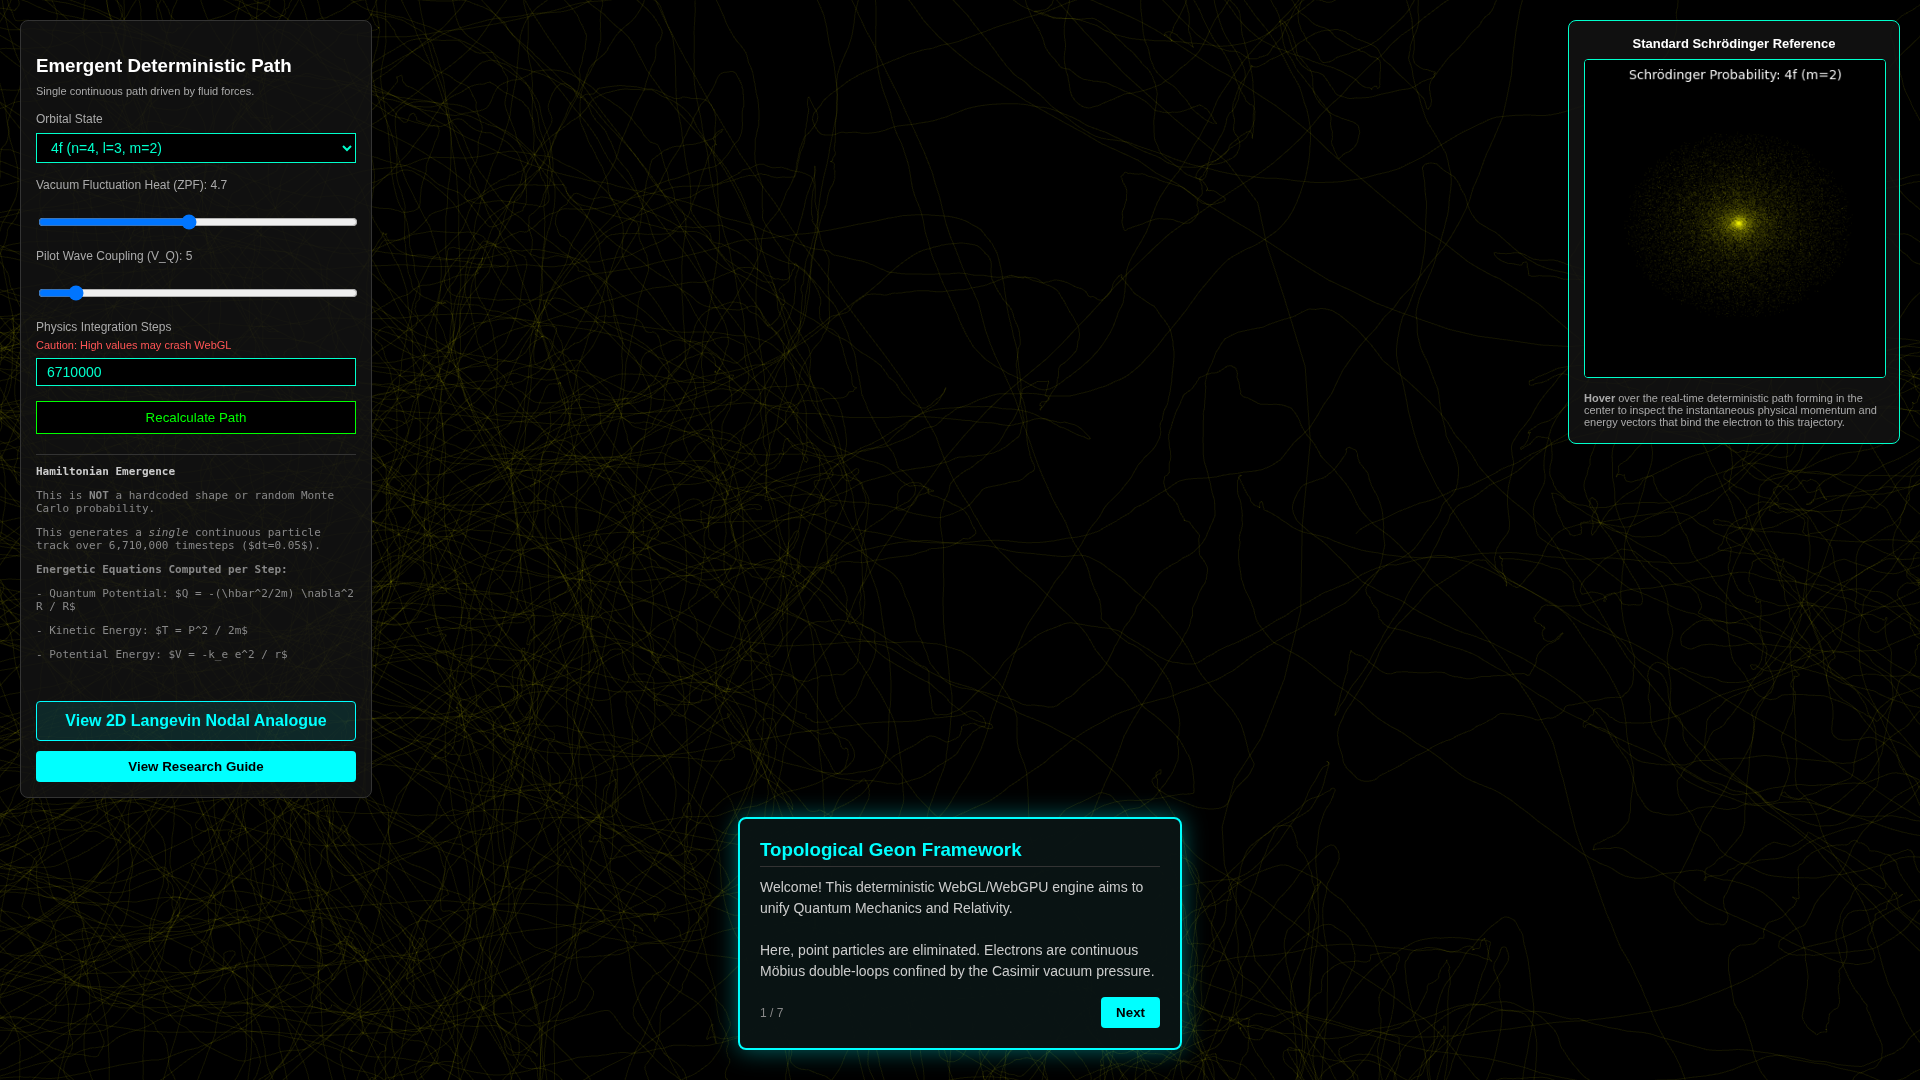
\includegraphics[width=\textwidth]{assets/4f_ergodic_weave.png}
    \caption{Deterministic weaving of the $4f$ orbital ($n=4, l=3, m=2$) using a Pilot Wave Coupling ($V_Q$) of $5.0$ and Vacuum Fluctuation Heat (ZPF) of $4.7$ over $6,710,000$ integration steps. The particle successfully explores all spatial lobes without becoming trapped at the nodal boundaries.}
    \label{fig:4f_weave}
\end{figure}

\end{document}
